\documentclass[twocolumn,10pt]{article}
\usepackage[ruled,linesnumbered]{algorithm2e}
\usepackage{graphicx}
\usepackage{amsmath}
\usepackage{algorithmicx}
\usepackage{algorithm}
\usepackage{url}
\usepackage{cite}
\usepackage{xcolor}
\usepackage{tikz}
\usetikzlibrary{arrows.meta, positioning, shapes.geometric}
\usepackage{booktabs}
\usepackage{tabularx}
\usepackage{listings}
\usepackage{hyperref}
\usepackage{comment}
\usepackage{float}

\hypersetup{
    colorlinks=true,
    linkcolor=blue,
    filecolor=magenta,      
    urlcolor=cyan,
    pdftitle={Hybrid Region Proposal and NLP-Based Approach for Handwritten Prescription Recognition},
    pdfauthor={Your Name},
}

\title{Medical Prescription Recognition for Efficient Healthcare Workflows}

\author{Nabeel Ahmed\\M240464CS\\Guided by: Sumesh TA}

\usepackage{epsfig}
\begin{document}
	
\maketitle
	
{\bf Keywords:}
Prescription Recognition, YOLOv8, TrOCR, Handwriting Recognition, Region Segmentation, Drug Lexicon, Data Augmentation


\begin{abstract}
Medication errors remain a critical healthcare concern, with illegible handwriting on prescriptions identified as a widely recognized cause of preventable harm \cite{statpearls2024, amcp2019}. Recent global estimates from the World Health Organization indicate that medication errors cause approximately one death per million population annually, which would translate to about 163,000 deaths per year in the European Union alone \cite{eaasm2022}.
This paper presents the current implementation of a region-aware handwritten prescription recognition framework. Unlike whole-document OCR systems, the proposed pipeline isolates handwritten prescription regions, segments them into line and word crops, recognizes medicine-name words using a fine-tuned TrOCR model, and validates the recognized text using dosage-frequency rules and drug-lexicon matching. The implementation includes notebook and Streamlit annotation tools, a YOLO-based handwritten-region cropper, a combined cropped-word TrOCR dataset, and train-time handwriting augmentation. In the latest Kaggle T4x2 fine-tuning run, \texttt{microsoft/trocr-base-handwritten} achieved 83.16\% strict exact-match accuracy, 89.06\% case-insensitive exact-match accuracy, 5.91\% character error rate, and 17.02\% word error rate on the validation split of the combined cropped-word dataset after 2500 training steps. The results show that transformer OCR is effective for medicine-name recognition when reliable word crops are available, while also emphasizing the importance of segmentation quality in full-prescription recognition.
\end{abstract}


\section{Introduction}
Prescription errors due to illegible handwriting remain a persistent challenge in healthcare delivery, with studies confirming approximately 7,000 deaths annually in the US alone due to misinterpreted prescriptions \cite{bhuiyan2022online}. Despite the push toward digital health records, 97.1\% of doctors in developing countries still rely on handwritten prescriptions due to time constraints and established habits \cite{bhuiyan2022online}. This creates a critical need for automated systems that can accurately interpret and digitize handwritten medical instructions.

The challenges of handwritten prescription recognition extend beyond general handwriting recognition problems due to several domain-specific factors:
\textbf{Mixed content documents}: Prescriptions typically contain both printed elements (headers, footers, pre-formatted fields) and handwritten content (medication names, dosages, instructions).\\
\textbf{Medical terminology}: Specialized vocabulary with complex spelling and abbreviations.\\
\textbf{Multilingual requirements}: Many prescriptions contain code-switching between English and regional languages \cite{irjmets2024}.\\
\textbf{Time-critical processing}: Delays in medication dispensing can impact patient care.



\section{Literature Survey}

\subsection{An Online Cursive Handwritten Medical Words Recognition System (Bhuiyan et al., 2022)}
This landmark study in Nature Scientific Reports \cite{bhuiyan2022online} addresses the critical challenge of handwritten prescription recognition in developing countries. The authors report that 97.1\% of Bangladeshi doctors still generate handwritten prescriptions, with illegibility causing adverse medical consequences including incorrect medications and improper dosing.

Key contributions include:
\textbf{Dataset Development}: Creation of 'Handwritten Medical Term Corpus' containing 17,431 samples of 480 medical terms
\textbf{RSS Data Augmentation}: Introduction of a novel Rotate-Shift-Stretch technique that expands the dataset to 1,591,100 samples
\textbf{Model Architecture}: Implementation of Bidirectional LSTM networks for sequence recognition
\textbf{Performance}: 93.0\% average accuracy (max: 94.5\%) with RSS augmentation


The RSS method transforms each stroke of a handwritten word by updating coordinates through rotation, shifting, and stretching operations, creating variations that better represent real-world handwriting diversity. This approach significantly outperformed previous methods such as SRP (Stroke Rotation and Parallel-shift), which achieved only 68.0\% accuracy \cite{bhuiyan2022online}.

\subsection{Handwritten Medical Term Recognition using Bidirectional LSTM}


Tabassum et al.~\cite{tabassum2022online} addressed the problem of illegible handwritten prescriptions in developing countries, where 97.1\% of doctors still rely on handwritten prescriptions due to time constraints. They developed a comprehensive system using Bidirectional LSTM networks for recognizing doctors' handwritten medical terminology. The authors created a specialized dataset called "Handwritten Medical Term Corpus" containing 17,431 samples of 480 medical terms (360 English and 120 Bangla) collected from 39 healthcare professionals. 

A key contribution of their work was the introduction of a novel data augmentation technique called RSS (Rotate-Shift-Stretch), which expanded their dataset to 1,591,100 samples by applying coordinate-based transformations to the handwriting strokes. Unlike traditional image-based approaches, their method processed sequence data representing pen movements, capturing the rich temporal information in handwriting. The system achieved 93.0\% average accuracy (max: 94.5\%, min: 92.1\%), which was 19.6\% higher than results without data augmentation. The authors proposed implementing this technology in a smartpen specifically designed for doctors, which would digitize handwritten prescriptions in real-time, potentially reducing medical errors and improving healthcare delivery in resource-constrained settings.

\subsection{Multilingual Prescription Recognition Using Deep Learning}

The work on multilingual prescription recognition systems demonstrates significant advancements in handling diverse language prescriptions:


    \textbf{Multi-language Support}: The system recognizes doctor's handwriting across multiple languages, addressing challenges in regions with linguistic diversity~\cite{pavithiran2024multilingual}
    \textbf{Hybrid Architecture}: Implements a combination of CNN, RNN, and LSTM techniques for improved recognition accuracy
    \textbf{Unicode Integration}: Utilizes Unicode mapping to handle various scripts and language characters
     \textbf{Post-processing Optimization}: Employs fuzzy search and market basket analysis with pharmaceutical databases to improve results
     \textbf{Image Pre-processing Pipeline}: Includes dedicated pre-processing and word segmentation before model training
     \textbf{Accuracy Performance}: Achieves approximately 89\% accuracy on multi-language prescription datasets


\subsection{Medical Handwritten Prescription Recognition and Information Retrieval Using Neural Network (2021)}
Utkarsh Shaw et al. \cite{utkarshaw2021} proposed a neural network-based system for recognizing handwritten medical prescriptions, particularly focusing on cursive handwriting1. The study utilized the Extended MNIST (EMNIST) dataset, which includes both digits and letters, to train a three-layer neural network. The architecture consists of an input layer with 785 units (784 features + bias), a hidden layer with 25 units, and an output layer with 10 units corresponding to target classes1. Preprocessing techniques such as grayscale conversion and segmentation were employed to prepare prescription images for recognition. Segmentation divided handwritten strokes into individual characters, resized to match the input dimensions of the neural network.

The model achieved a training accuracy of 94.49\% and a test accuracy of 80.72\%, demonstrating its effectiveness in recognizing cursive handwriting1. Practical applications include extracting medicine names from prescriptions, historical document recognition, postal code identification, and real-time handwriting conversion. Minor misclassifications were observed due to similarities in character shapes (e.g., "5" misclassified as "S"), which the authors plan to address by employing deeper neural networks and more comprehensive datasets in future iterations.

\section{Problem Statement}
Handwritten medical prescriptions are difficult to digitize due to inconsistent handwriting, mixed printed and handwritten regions, and frequent image quality issues. These challenges make it hard to accurately extract medication details and can lead to serious dispensing errors, as highlighted by Bhuiyan et al. \cite{bhuiyan2022online}. This project aims to develop a reliable end-to-end system that can segment prescription regions, recognize handwritten text, and validate extracted information to support safer and more efficient healthcare workflows.



\section{Proposed Methodology}

\subsection{System Architecture}
Our system employs a five-stage modular pipeline as illustrated in Figure \ref{fig:architecture}:

\begin{figure}[H]
\centering
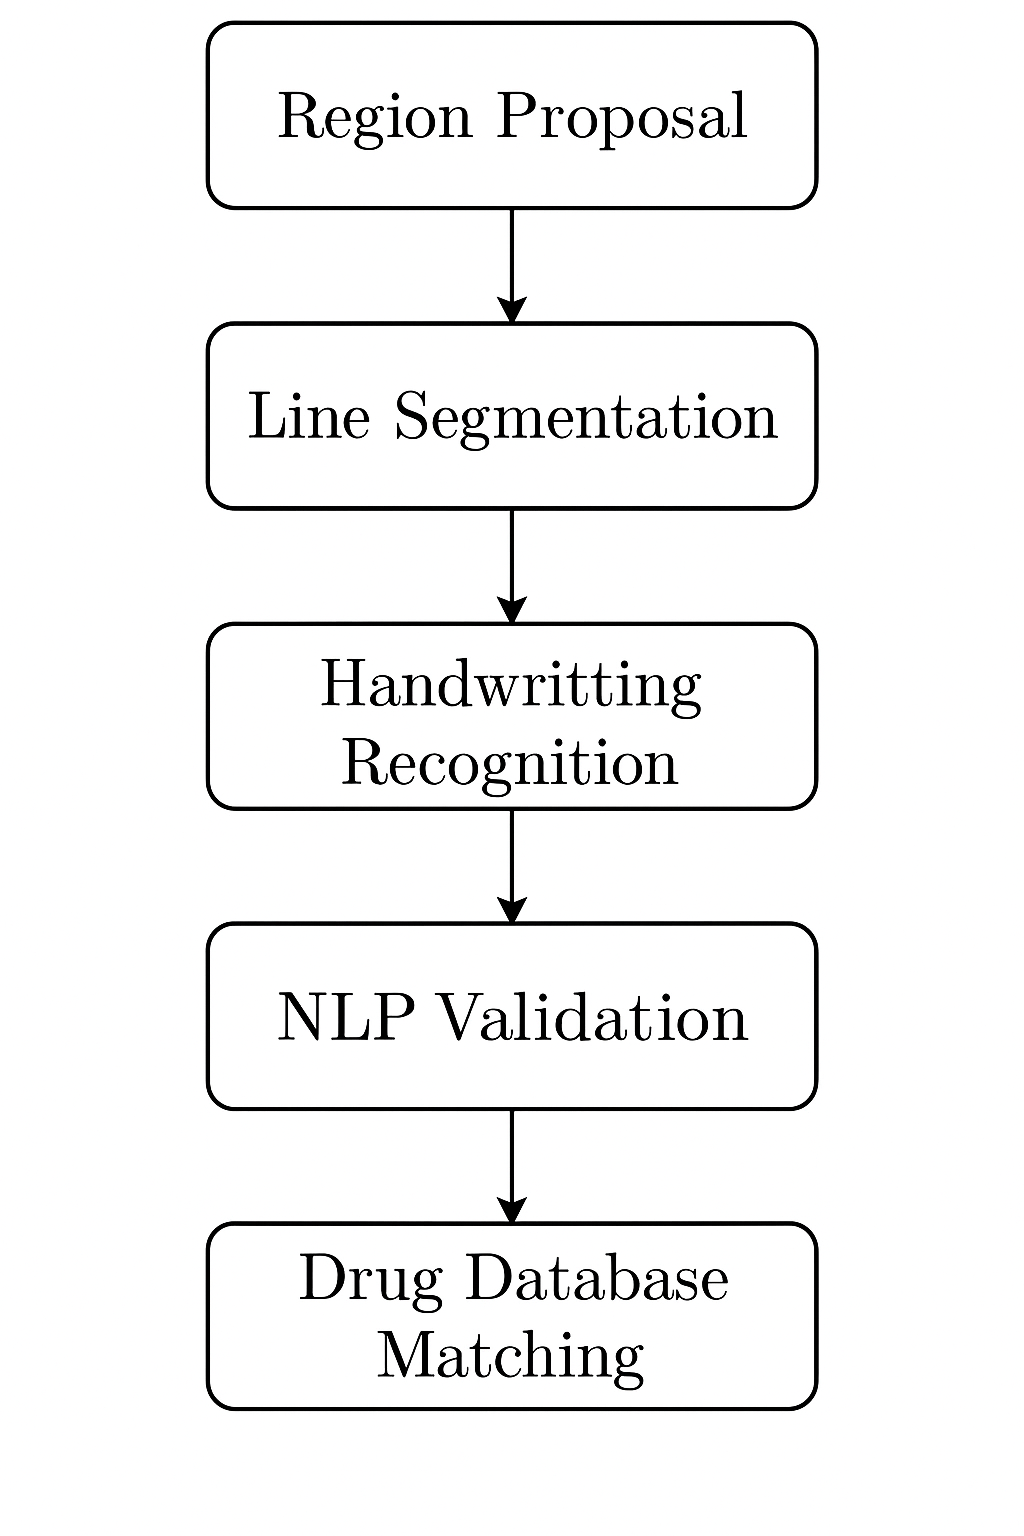
\includegraphics[width=0.95\columnwidth]{architecture}
\caption{Pipeline: preprocessing, region segmentation, line and word segmentation, OCR with TrOCR, and validation using rules and lexicon matching.}
\label{fig:architecture}
\end{figure}

\begin{figure*}[t]
\centering
\begin{tikzpicture}[
  node distance=7mm and 8mm,
  block/.style={draw, rounded corners, align=center, minimum height=9mm, text width=0.18\textwidth, font=\small},
  arrow/.style={-{Latex[length=2mm]}, thick}
]
\node[block] (raw) {Raw prescription\\photograph};
\node[block, right=of raw] (pre) {Preprocessing\\illumination and\\contrast normalization};
\node[block, right=of pre] (region) {YOLO\\handwritten-region\\detector};
\node[block, right=of region] (seg) {Line and word\\segmentation};
\node[block, right=of seg] (ocr) {Fine-tuned\\TrOCR word\\recognition};
\node[block, below=of ocr] (valid) {Dosage-frequency\\rules and drug\\lexicon matching};
\draw[arrow] (raw) -- (pre);
\draw[arrow] (pre) -- (region);
\draw[arrow] (region) -- (seg);
\draw[arrow] (seg) -- (ocr);
\draw[arrow] (ocr) -- (valid);
\end{tikzpicture}
\caption{Implemented full-prescription inference flow from a raw prescription image to validated medicine-name predictions.}
\label{fig:implemented-flow}
\end{figure*}

Unlike traditional OCR systems, our approach treats each prescription zone independently. This modularity allows each component to be optimized for its sub-task (e.g., handwritten medicine vs. printed header).
\subsection{Data Acquisition and Preparation}

\subsubsection{Datasets}
The OCR training set combines the Doctor's Handwritten Prescription BD dataset with two additional cropped medicine-word datasets added during the current phase. The merged dataset contains 8274 training samples, 1033 validation samples, and 1040 testing samples before augmentation. The full-prescription side of the project uses custom prescription photographs collected for pipeline development and annotation. These raw pages are converted into region crops, line crops, word crops, and manifest files by the implemented preprocessing and annotation tools.


\subsubsection{Dataset Organization}
Data is stored in a structured format:

\texttt{data/combined\_trocr\_word\_dataset/}: cropped word images and split CSV files for TrOCR training, validation, and testing.\\
\texttt{data/processed/regions/}: handwritten-region crops and manifests.\\
\texttt{data/processed/line\_crops/} and \texttt{data/processed/word\_crops/}: intermediate crops used for OCR and review.\\
\texttt{models/}: stable YOLO and TrOCR model outputs.\\
\texttt{lexicons/}: drug-name candidates for fuzzy validation.


\subsubsection{Dataset Size Targets}

The current combined OCR dataset contains more than ten thousand labelled word crops before train-time augmentation. The page-level dataset is still smaller and is used primarily to train and validate the handwritten-region cropper and to generate additional reviewed word crops through the annotation workflow.


\subsection{Preprocessing and Privacy}
Prescription images undergo grayscale conversion, illumination compensation, contrast normalization, thresholding, and connected-component processing where needed. Region and word crops are stored with manifests so that each prediction can be traced back to its source image. Patient-identifying information is not used as an OCR target; privacy-preserving masking is retained as a deployment requirement before larger-scale annotation.

\subsection{Region Segmentation Module}
The current implementation uses a YOLO detector for handwritten-region bounding boxes rather than whole-page OCR. Manual region corrections are exported into a YOLO-format dataset and used to train a lightweight detector for the \texttt{handwritten\_region} class. This detector replaces the earlier heuristic cropper and produces stable region crops for subsequent line and word segmentation. In the latest region-detection run, the validation result reached 99.40\% precision, 100.00\% recall, 99.50\% mAP@0.5, and 92.90\% mAP@0.5:0.95 on the small validation split.

\subsection{Line Segmentation}
Handwritten zones are further segmented into line and word crops using OpenCV-based projection profiles, morphological operations, contour filtering, and crop normalization. The final OCR unit is a word crop because the trained TrOCR model predicts medicine-name words. Manual correction tools are provided for cases where automatic line or word segmentation merges multiple words or misses faint handwriting.

\subsection{Handwriting Recognition}
We employ \textbf{TrOCR}, a transformer-based OCR model, fine-tuned on the combined cropped medicine-word dataset. The model is trained for the \texttt{MEDICINE\_NAME} target using train-only augmentation, including small rotation, translation, scaling, contrast variation, blur, and noise. The current notebook trains the full encoder-decoder model, uses beam search during evaluation, and selects the best checkpoint using exact-match accuracy.

\subsection{Transformer Adaptation}
The contribution is not a new transformer architecture; it is the prescription-domain adaptation workflow built around pretrained TrOCR. The pretrained model is adapted through the combined medicine-word dataset, train-only handwriting augmentation, full encoder-decoder fine-tuning, explicit decoder-input preparation for stable training in the current Transformers environment, beam-search decoding, checkpoint selection by exact-match accuracy, and post-OCR lexicon/rule validation.

\begin{figure*}[t]
\centering
\begin{tikzpicture}[
  node distance=6mm,
  block/.style={draw, rounded corners, align=center, minimum height=8mm, text width=0.74\textwidth, font=\small},
  arrow/.style={-{Latex[length=2mm]}, thick}
]
\node[block] (base) {Pretrained \texttt{microsoft/trocr-base-handwritten}: vision encoder + autoregressive text decoder};
\node[block, below=of base] (data) {Prescription-domain data: combined medicine-word dataset + train-time handwriting augmentation};
\node[block, below=of data] (train) {Fine-tuning changes: full encoder-decoder training, explicit decoder inputs, best checkpoint by exact match};
\node[block, below=of train] (decode) {Inference and validation: beam search, text normalization, dosage-frequency rules, drug lexicon matching};
\draw[arrow] (base) -- (data);
\draw[arrow] (data) -- (train);
\draw[arrow] (train) -- (decode);
\end{tikzpicture}
\caption{Adaptation applied around the pretrained TrOCR transformer for medicine-name recognition.}
\label{fig:trocr-adaptation}
\end{figure*}

\subsection{NLP Validation}
The current validation layer uses regular expressions to extract dosage and frequency expressions and fuzzy matching to compare OCR outputs against a medicine lexicon. BioBERT is kept as a future extension for biomedical named-entity recognition; it is not required for the current implemented OCR results.

\section{Phase 4 Results (Implemented Module)}
In this phase, we implemented the end-to-end region-aware pipeline components and trained the word-level OCR module. The OCR result reported here is from the latest Kaggle T4x2 TrOCR run on the validation split of the combined cropped prescription-word dataset. The run used train-time augmentation and trained for 2500 steps, approximately 1.61 epochs over the augmented training set.

\begin{table}[h]
\centering
\caption{Current Phase 4 TrOCR Validation Results}
\label{tab:phase4_ocr_results}
\renewcommand{\arraystretch}{1.2}
\small
\begin{tabularx}{\columnwidth}{Xr}
\toprule
\textbf{Metric} & \textbf{Value} \\
\midrule
Strict Exact-Match Accuracy & 83.16\% \\
Case-Insensitive Exact-Match Accuracy & 89.06\% \\
Character Error Rate (CER) & 5.91\% \\
Word Error Rate (WER) & 17.02\% \\
Validation Loss & 0.2076 \\
Training Steps & 2500 \\
Validation Samples & 1033 \\
\bottomrule
\end{tabularx}
\end{table}

The validation metrics improved consistently during training. Strict exact-match accuracy increased from 73.18\% at step 500 to 83.16\% at step 2500, while CER decreased from 9.39\% to 5.91\%. The case-insensitive score is higher because many errors are capitalization differences that can be normalized safely before lexicon validation. The result is lower than the earlier single-dataset presentation result because the current combined dataset is larger, more varied, and more realistic.

\section{Conclusion}
The proposed region-aware handwritten prescription recognition framework addresses limitations of traditional whole-document OCR. By integrating YOLO-based handwritten-region detection, OpenCV-based line and word segmentation, TrOCR-based medicine-name recognition, and rule-plus-lexicon validation, the system provides a practical modular workflow for complex prescription documents.

Data augmentation and preprocessing enhance model generalization, while modular design ensures efficiency by focusing computation on relevant zones. The current implementation uses YOLO region detection, OpenCV line and word segmentation, word-level TrOCR recognition, and rule-plus-lexicon validation. Future work will complete test-set evaluation from the saved best TrOCR checkpoint, expand the reviewed full-page dataset, quantitatively evaluate page-level region and word segmentation, explore few-shot learning to reduce annotation costs, and integrate with electronic health record systems.

If successful, this system could reduce prescription interpretation errors and mitigate preventable adverse drug events, providing a practical AI-driven solution to a pressing healthcare challenge.

\bibliographystyle{unsrt}
\bibliography{references}

\end{document}
